\documentclass[twocolumn]{article}

\usepackage{enumerate}
\usepackage{graphicx}
\usepackage[colorlinks=true,linkcolor=blue]{hyperref}
\usepackage[table,xcdraw]{xcolor}
\usepackage[english,spanish]{babel} 
\usepackage{helvet}

\renewcommand{\familydefault}{\sfdefault}

\newenvironment{poliabstract}[1]
   {\renewcommand{\abstractname}{#1}\begin{abstract}}
   {\end{abstract}}

\begin{document}

\title{Comparativa de gestores de bases de datos no relacionales}
\author{Lipa Calabilla, Abraham\\Herrera Amezquita,
Derian  \\Paredes Catacora, Randi \\Mejia Rodriguez, Julio}


\date{30 de Noviembre de 2020}

\maketitle

\selectlanguage{spanish}
\begin{poliabstract}{Resumen} 
  Como su propio nombre indica, las bases de datos no 
  relacionales son las que, a diferencia de las relacionales,
   no tienen un identificador que sirva de relación entre un 
   conjunto de datos y otros. Como veremos, la información
    se organiza normalmente mediante documentos y es muy
     útil cuando no tenemos un esquema exacto de lo que se va a almacenar.

     Las bases de datos NoSQL están diseñadas específicamente
     para modelos de datos específicos y tienen esquemas flexibles 
     para crear aplicaciones modernas. Las bases de datos NoSQL son 
     ampliamente reconocidas porque son fáciles de desarrollar, por 
     su funcionalidad y el rendimiento a escala.
  
\end{poliabstract}

\selectlanguage{english}
\begin{poliabstract}{Abstract} 
  As the name suggests, databases do not
  relational are those that, unlike relational,
   do not have an identifier that serves as a relationship between a
   data set and others. As we will see, the information
    is normally organized by documents and is very
     useful when we do not have an exact schematic of what to store.

     NoSQL databases are specifically designed
     for specific data models and have flexible schemas
     to create modern applications. NoSQL databases are
     widely recognized because they are easy to develop, for
     its functionality and performance at scale.
\end{poliabstract}

\section{Introducción}
Las bases de datos relacionales dominaron el 
mundo de la gestión de datos desde la década de los 
70, pero al surgir el  Internet y su auge como 
plataforma del desarrollo de aplicaciones pusieron a prueba  el dominio de las 
soluciones relacionales.

El volumen de datos al que debe hacer frente una aplicación web 
ha crecido exponencialmente durante los últimos años, así como el 
número de usuarios que utiliza las aplicaciones 
disponibles en Internet, y en consecuencia el volumen de transacciones 
y la demanda a la que se ven sometidas, ya que los usuarios esperan un
 tiempo de respuesta inmediato en sus interacciones online con el website.
 En el presente trabajo desarrollaremos mas a fondo los distintos temas
 acerca de las bases de datos no relacionales.


\section{Bases de datos}

Una base de datos no es nada más que una colección de información que existe a lo largo de un periodo de tiempo, generalmente por muchos años.

El término ``database" se refiere a una colección de datos que son manejados por un \textit{Sistema gestor de base de datos} (o simplemente, Gestor de base de datos o \textbf{DBMS}). [1]

De un DBMS se espera:

\begin{itemize}
  \item Que los usuarios puedan crear nuevas bases de datos, consultar y modificar los datos ubicados en éstas, usando un lenguaje de definición, de consultas y de manipulación de datos, respectivamente.
  \item Que soporten el almacenamiento de grandes cantidades de información, así como la persistencia, el acceso eficiente y la recuperación.
  \item Que controle el acceso a los datos otorgado a los usuarios y que evite las acciones parciales sobre los datos.
\end{itemize}

Las bases de datos tradicionales están siendo utilizadas desde los 70's y su trabajo consiste en almacenar una gran cantidad de datos y obteniendo datos de múltiples tablas mediante uniones (\textit{`joins'}) complejas. [2]

Por 1990, las bases de datos relacionales fueron la norma. Las operaciones realizadas sobre los datos de una base de datos relacional se podían realizar mediante SQL (Lenguaje Estructurado de Consultas), el cual fue el más importante basado en el modelo relacional. [1]

\section{Bases de datos no relacionales}

\begin{description}
  \item[NoSQL] Se refiere a `No solo SQL' o simplemente `No SQL'. Describe tecnologías para el almacenamiento de datos que permiten la persistencia de datos con un alto rendimiento necesario para las aplicaciones de la escala de Internet de la actualidad. [3]
\end{description}

Una base de datos no relacional (o bases de datos NoSQL) responde a las necesidades de desarrollo de las aplicaciones modernas. [4]

\begin{itemize}
  \item Las aplicaciones generan enormes volúmenes de datos nuevos y en constante evolución (estructurados, semiestructurados, no estructurados y polimórficos).
  \item El trabajo se realiza en equipos pequeños, que realizan `sprints' de desarrollo ágiles con iteraciones rápidas.
  \item Las aplicaciones sirven como servicios, que no solo deben funcionar sin interrupción, sino que además tienen que ser accesibles desde muchos dispositivos distintos y deben poder escalarse.
  \item Las organizaciones ahora están recurriendo a arquitecturas de escalamiento horizontal que utilizan tecnologías de software abierto, servidores básicos y computación en la nube.
\end{itemize}

\subsection{Tipos de bases de datos NoSQL}

\begin{enumerate}

  \item Clave/Valor \\
        Los datos usan claves que son identificadores y que son similares a una llave primaria en una
         base de datos relacional. [3] Cada elemento de la base de datos se almacena como un nombre
          de atributo (o clave), junto con su valor. [4] Algunos ejemplos de este tipo son \textbf{Riak } y \textbf{Berkeley DB}.

  \item Orientadas a columnas \\
        Los datos se organizan por columnas en lugar de por filas. 
        El efecto de este diseño arquitectónico es que hace que las
         consultas agregadas sobre grandes cantidades de datos sean mucho más
          rápidas de procesar. [3] Algunos ejemplos de este tipo son \textbf{Cassandra} y \textbf{HBase}.

  \item Documentos \\
        Se empareja cada clave con una estructura de datos
         compleja que se denomina `documento'. Los documentos 
         pueden contener muchos pares de clave-valor distintos, 
         o pares de clave-matriz, o incluso documentos anidados. [4] Un ejemplo de este tipo es \textbf{MongoDB}.

  \item Grafos \\
        Utilizan la teoría de grafos para almacenar relaciones 
        de datos en una serie de vértices con aristas, lo que 
        hace que las consultas que funcionen con datos de esta 
        manera sean mucho más rápidas. [3] Algunos ejemplos de este tipo son \textbf{Neo4J} y \textbf{Giraph}.

\end{enumerate}

\section{MongoDB}

MongoDB es una base de datos NoSQL basado en documentos JSON y de código abierto escrito en C++, que proporciona alto rendimiento, alta disponibilidad y escalabilidad automática. [5]

Las bases de datos como MongoDB proporcionan escalabilidad automática, lo cual hace que esta base de datos sea idónea para grandes cantidades crecientes de información. [5]

El desarrollo de MongoDB comenzó en el año 2007 por la empresa 10gen3, publicando una versión final en el 2009 y actualmente se encuentra en la versión 4.4. [5]

\subsection{RDBMS y MongoDB}

A continuación se muestra una comparación de los términos utilizados en ambos tipos de bases de datos solo a modo orientativo, dado que no cuentan con la misma estructura. [6]

\begin{table}[h]
\centering
\begin{tabular}{|l|l|}
\hline
\rowcolor[HTML]{67FD9A} 
\textbf{RDBMS} & \textbf{MongoDB}               \\ \hline
Database       & Database                       \\ \hline
Table          & Collection                     \\ \hline
Tuple/Row      & Document                       \\ \hline
Column         & Field                          \\ \hline
Table Join     & Embedded Documents             \\ \hline
Primary Key    & Primary Key (Default key \_id) \\ \hline
\end{tabular}
\caption{Tabla comparativa de terminología RDMS - MongoDB}
\end{table}

\subsection{Ventajas sobre RDBMS}

Algunas de las ventajas que tiene MongoDB sobre los gestores de bases de datos relacionales son: [6]

\begin{itemize}
  \item Menos esquema
  \item La estructura de un objeto es clara
  \item No requiere de uniones complejas
  \item Consultas dinámicas sobre documentos
  \item Fácil escalabilidad
  \item No requiere de conversión o mapeo de objetos
  \item Rápido acceso a los datos
\end{itemize}

\subsection{Arquitectura}

En una base de datos de MongoDB, hay tres partes principales: [8]

\begin{description}
  \item[mongod (MongoDB server)] Es el proceso principal que maneja las solicitudes de datos, administra el formato de los datos y realiza operaciones de administración en segundo plano. Puede haber muchos demonios mongod ejecutándose como instancias primarias secundarias.
  \item[mongos] Es el servicio de enrutamiento. Este proceso enruta información y datos en el clúster.
  \item[MongoDB shell] Es la interfaz interactiva. Al usar JavaScript para ordenar, el desarrollador puede examinar los resultados de las consultas y verificar los casos de prueba.
\end{description}

\begin{figure}[h]
  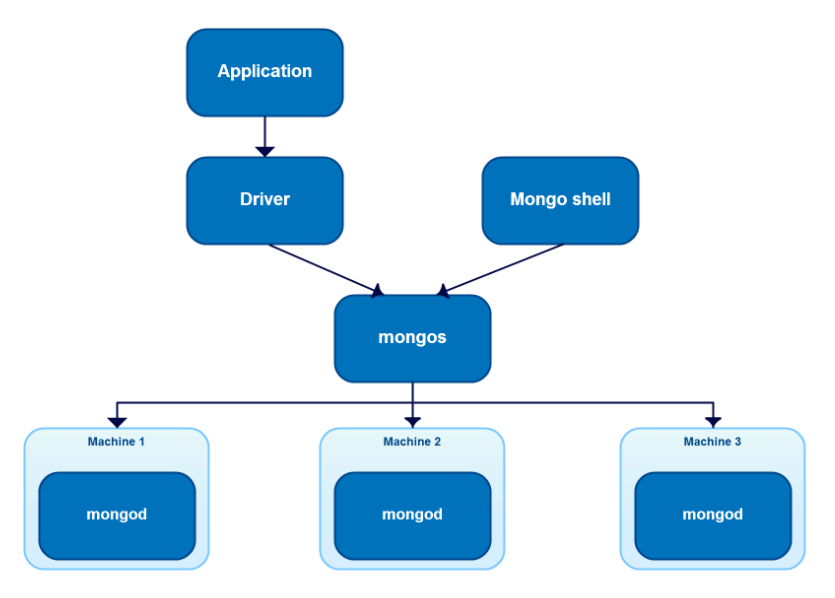
\includegraphics[width = \columnwidth]{img/01_mongo.png}
  \caption{Arquitectura de una base de datos MongoDB}
\end{figure}

\subsection{BSON}

Generalmente, los usuarios trabajan con MongoDB mediante el formato JSON, sin embargo, MongoDB usa BSON (o `Binary JSON'). BSON extiende del modelo JSON para proporcionar ``tipos de datos" para una correcta codificación y decodificación en los diferentes lenguajes. [5]

\subsubsection{JSON y BSON}

JSON proporciona únicamente 6 tipos de datos: [5]

\begin{itemize}
  \item String
    \\ Este tipo de dato lo compone una cadena de texto normal.
  \item Number
    \\Este tipo de dato lo compone un número par o impar, se declara sin comillas dobles.
  \item Booleans
    \\Este tipo de dato es utilizado como una opción de tipo true o false.
  \item null
    \\Sencillamente este dato es para dejar en blanco los valores de un dato.
  \item Arrays
      \\Este tipo de datos es para crear un nuevo subconjunto de datos independientes dentro del JSON.  
  \item Objetos / documentos
      \\Un archivo JSON puede tener objetos, es decir una nueva fila que dentro de ella hay un conjunto de datos específicos.
\end{itemize}

Los tipos de datos que maneja internamente BSON son los siguientes:

\begin{itemize}
  \item Double
  \\Representa un valor flotante.
  \item String
  \\Las cadenas BSON son UTF-8. En general,
   los controladores para cada lenguaje de 
   programación se convierten del formato de 
   cadena del lenguaje a UTF-8 al serializar y 
   deserializar BSON. Esto hace posible almacenar 
   la mayoría de los caracteres internacionales en cadenas 
   BSON con facilidad.

  \item Object
  \\Representa un documento incrustado.
  \item Array
  \\Los conjuntos o listas de valores se pueden representar como matrices.
  \item Binary data
  \\Los datos binarios son una cadena de bytes arbitrarios, no se pueden manipular desde el shell.
  \item Undefined (deprecated)
  \item Object id
  \\Los ObjectIds (identificador de documento MongoDB, equivalente a una clave principal) son: pequeños, probablemente únicos, rápidos de generar y ordenados. Estos valores constan de 12 bytes, donde los primeros cuatro bytes son una marca de tiempo que refleja la creación del ObjectId.
  
  \item Boolean
 \\ Un verdadero o falso lógico. Se usa para evaluar si una condición es verdadera o falsa
  \item Date
 \\ BSON Date es un entero de 64 bits que representa el número de milisegundos desde la época de Unix (1 de enero de 1970).
  \item Null
  \\Representa tanto un valor nulo como un campo inexistente.
  \item Regular Expression
  
  \item JavaScript Symbol JavaScript (con scope)
  
  \item 32-bit integer
  \\Los números sin puntos decimales se guardarán como enteros de 32 bits.
  \item Timestamp
  \\BSON tiene un tipo de marca de tiempo especial para el uso interno de MongoDB y no está asociado con el tipo de fecha normal.
  \item 64-bit integer
  \\Los números sin punto decimal se guardarán y se devolverán como enteros de 64 bits.
  \item Min key
  \\MinKey compara menos que todos los demás valores posibles de elementos BSON, respectivamente, y existen principalmente para uso interno.
  \item Max key
  \\MaxKey compara más que todos los demás valores posibles de elementos BSON, respectivamente, y existen principalmente para uso interno.s
\end{itemize}

\section{Redis}

Redis es una base de datos NoSQL, pero también, es una base de datos multi-modelo que permite la búsqueda, la mensajería, streaming, grafos y otras capacidades más allá de la de un simple almacén de datos. [3]

Redis mantiene los datos en la memoria para un acceso rápido y conserva los datos en el almacenamiento, así como la replicación de los contenidos en la memoria para escenarios de producción de alta disponibilidad. [3]

\subsection{Estructura}

\subsubsection{Bases de datos}

En Redis, al igual que en otras DBMS, una base de datos es un conjunto de datos. El caso de uso típico para una base de datos es agrupar los datos de una aplicación y mantenerlos separados de otras aplicaciones. [7]

\subsubsection{Clave / Valor}

Cada una de las estructuras de datos en Redis tienen al menos una clave y un valor. [7]

\begin{description}
  \item[Claves] Son cómo identificamos piezas de datos.
  \item[Valor] Representan los datos actualmente asociados con la clave.
\end{description}

\subsection{Almacenamiento de estructuras de datos}

Las estructuras de datos soportadas que se incluyen: [3]

\begin{itemize}
  \item Strings
  \\En Redis un string es una secuencia de bytes, lo que nos permite almacenar cualquier dato, como cadenas de texto, números, imágenes, vídeos, o un objeto serializado.
  \item Lists
  \\Las listas permiten almacenar secuencias de strings en el orden en el que fueron insertadas. En Redis las listas están optimizadas para que añadir un elemento al inicio o al final de la lista tarde lo mismo independientemente de si la lista tiene 10 elementos, o 100 millones de elementos.
  \item Sets
  \\Los sets son colecciones de strings, sin ningún orden particular, en los que se garantiza que los elementos del mismo son únicos y no pueden estar duplicados. Podemos añadir el mismo elemento 10 veces, pero Redis garantiza que sólo existirá una vez, lo que nos permite poder añadir elementos sin tener que preocuparnos previamente de si ya existen o no.
  \item Sorted sets
 \\Permiten la ordenación de los elementos en base a un valor (score) numérico asociado a cada uno de ellos. Es importante aclarar que la unicidad de los elementos se hace sólo teniendo en cuenta los datos almacenados, y no el valor del score. Si se añade el mismo elemento varias veces con distintos valores del score, el elemento sólo existirá un vez, y el score será el de la última actualización.
  \item Hashes
  \\Permite asociar a una clave una colección de pares clave-valor, habitualmente usado para representar objetos.
  \item Bit arrays
  
  \item Streams
  
  \item HyperLogLogs
\\Es una estructura de datos probabilística que se utiliza para contar valores únicos, o como se le conoce en matemáticas: calcular la cardinalidad de un conjunto.
\end{itemize}

\subsection{Arquitectura}

La arquitectura de Redis está basada en el enfoque BASE (Disponible básicamente, Soft-state y eventualmente consistente) mientras se elimina el enfoque ACID (atomicidad, consistencia, durabilidad y aislamiento) en RDBMS. Redis se basa en la arquitectura cliente / servidor y consta de los siguientes componentes: [8]

\begin{itemize}
  \item Servidor Redis
  \item Servidores réplica de Redis (opcionales)
  \item Cliente Redis
\end{itemize}

\begin{figure}[h]
  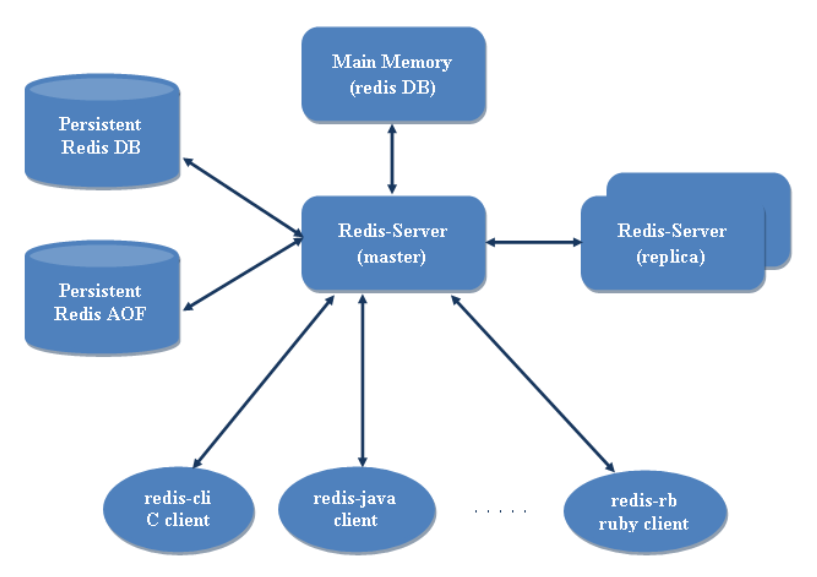
\includegraphics[width = \columnwidth]{img/02_redis.png}
  \caption{Arquitectura de una base de datos Redis}
\end{figure}

\section{Rendimiento}

Para la comparación de rendimiento entre MongoDB y Redis, se ha realizado un proceso de benchmarking en una sola máquina (con las mismas características). La herramienta utilizada es YCSB (Yahoo Cloud Serving Benchmark).

Versiones de las bases de datos:

\begin{description}
  \item[MongoDB] 2.7.4
  \item[Redis] 2.8.15
\end{description}

Se muestran los datos correspondientes a la relación entre el número de hilos de la máquina (los cuales son 1, 2, 4 y 8) y las operaciones por segundo, dada cierta cantidad de registros (1000, 5000 y 10000) y 1000 operaciones realizadas.

\begin{figure}[h]
  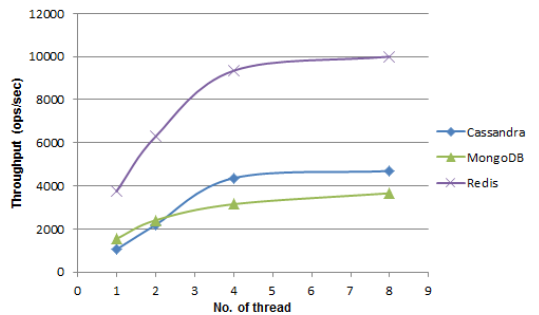
\includegraphics[width = \columnwidth]{img/03_g1.png}
  \caption{Gráfico comparativo con 1000 registros y 1000 operaciones}
\end{figure}

\begin{figure}[h]
  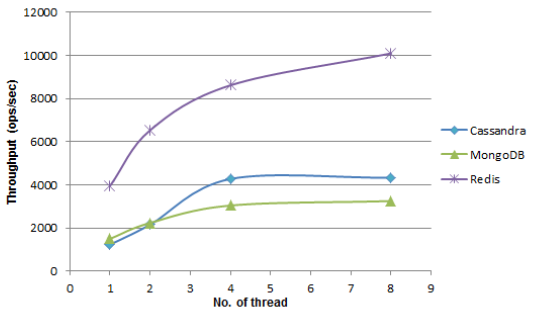
\includegraphics[width = \columnwidth]{img/04_g2.png}
  \caption{Gráfico comparativo con 5000 registros y 1000 operaciones}
\end{figure}

\begin{figure}[h]
  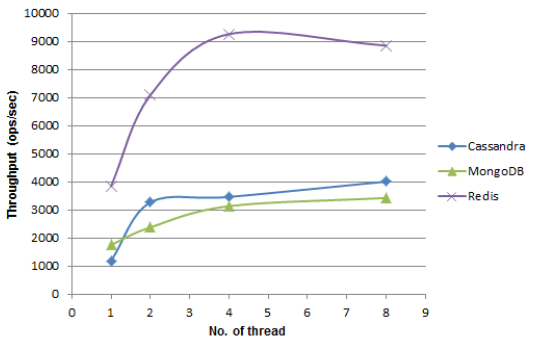
\includegraphics[width = \columnwidth]{img/05_g3.png}
  \caption{Gráfico comparativo con 10000 registros y 1000 operaciones}
\end{figure}

\newpage
\section{Conclusiones}
A partir de la definición, requisitos, ventajas 
y características de la base de datos no relacionales, podemos 
conocer algunos aspectos dignos de atención, entre ellos
 podemos decir que la base de datos: una base de datos es 
 un conjunto de datos o información que se utiliza para brindar servicios para muchas aplicaciones al mismo tiempo. En cuanto a los requisitos, se puede decir que ha realizado las mismas tareas de análisis que el software, y tiene las características de asociar información en organizaciones y asociaciones La ventaja de la base de datos es que la plataforma se puede utilizar para desarrollar aplicaciones. organización. Otro aspecto importante es el diseño y creación de la base de datos, existen muchas formas de organizar la información y expresar la relación entre los datos, los tres modelos lógicos principales en la base de datos son jerárquico, de red y relacional. Tiene ciertas ventajas comerciales y de procesamiento.


\section{Recomendaciones}

La elección de la tecnología de almacenamiento
 adecuada implica muchas consideraciones. Aunque 
 el rendimiento suele ser el factor más importante,
  se deben considerar factores como la funcionalidad, 
  la facilidad de operación, la facilidad de uso, la 
  disponibilidad de profesionales conocedores, la seguridad 
  y otros factores (como la existencia de herramientas y las 
  comunidades que respaldan el producto).
   Gracias a los beneficios como el aumento de 
   la productividad del equipo de desarrollo, la capacidad 
   de ingresar al mercado antes y reducir el costo total de
    propiedad, vemos cómo la tecnología NoSQL se convierte 
    cada vez más en parte de las soluciones de proyectos 
    comerciales.
    Es importante tener en cuenta que, como dice el nombre "NoSQL", no solo SQL
     ("no solo SQL"), las tecnologías NoSQL no son necesariamente la única parte 
     del almacenamiento de datos de la solución, pero a menudo acompañan a las bases
      de datos SQL, incluso si siguen siendo seguras en el futuro Úselo, incluso en 
      combinación con otras bases de datos NoSQL.
      Con el reciente crecimiento explosivo de las arquitecturas
       basadas en microservicios, veremos cada vez más cómo cada 
       servicio encapsula su propia solución de gestión de datos y, 
       en la mayoría de los casos, utiliza ciertas tecnologías NoSQL disponibles.



\section{Bibliografía}

\begin{thebibliography}{X}
  \bibitem{Baz} \textsc{Garcia\-Molina, H., Ullman, J., \& Widom, J. } ,
  \textit{}(2008),Database Systems: The Complete Book (2.a ed.). Pearson.
  
  \bibitem{Baz} \textsc{Punia, Y., \& Aggarwal, R. } ,
  \textit{}(2014),Implementing Information System Using MongoDB and Redis. International Journal of Advanced Trends in Computer Science and Engineering,3(2), 16-20.
  
  \bibitem{Baz} \textsc{John Wiley \& Sons, Inc.  } ,
  \textit{}(2019),Redis For Dummies(Limited Edition) [Libro electrónico]. John Wiley \& Sons, Inc. \url{https://redislabs.com/redis-for-dummies/}

  \bibitem{Baz} \textsc{MongoDB. (s. f.).} ,
  \textit{}Explicación sobre las bases de datos NoSQL. Recuperado 1 de diciembre de 2020, de:\url{https://www.mongodb.com/es/nosql-explained}

  \bibitem{Baz} \textsc{Madrigal Marinas, J. M. M. } ,
  \textit{}(2020), MongoDB en Castellano (2020.a-07-13 ed. ed.) [Libro electrónico]. Leanpub. \url{https://leanpub.com/mongodbcastellano}

  \bibitem{Baz} \textsc{Tutorials Point (I) Pvt. Ltd.} ,
  \textit{}(2018),MongoDB Tutorial. Tutorials Point (I) Pvt. Ltd. \url{https://www.tutorialspoint.com/mongodb/mongodb_tutorial.pdf}

  \bibitem{Baz} \textsc{Karl Seguin, K. S. } ,
  \textit{}(2020),The Little Redis Book (1.a ed.) [Libro electrónico]. Github. \url{https://github.com/karlseguin/the-little-redis-book}

  \bibitem{Baz} \textsc{Kumarasinghe, C. U., Liyanage, K. L. D. U., Madushanka, W. A. T., \& Mendis, R. A. C. L. } ,
  \textit{}(2016),Performance Comparison of NoSQL Databases in Pseudo Distributed Mode: Cassandra, MongoDB \& Redis.

\newpage
  \bibitem{Baz} \textsc{GoalKicker.com.  } ,
  \textit{}(2017),MongoDB Notes for Professionals (3.6.1 ed.) [Libro electrónico]. GoalKicker.com. \url{https://goalkicker.com/MongoDBBook/MongoDBNotesForProfessionals.pdf}

\end{thebibliography}


\end{document}